% ====================================================================
%  Gaia DR3 5870569352746778624: A ~12.5 M_sun Stellar-Mass
%  Black Hole Candidate in the Galactic Disk from Combined
%  Astrometric and Spectroscopic (AstroSpectroSB1) Orbital Solution
%  MNRAS format — single-target focused paper
% ====================================================================
\documentclass[usenatbib,fleqn]{mnras}

\usepackage{amsmath,amssymb}
\usepackage{graphicx}
\usepackage{booktabs}
\usepackage{natbib}
\usepackage{hyperref}
\usepackage{xcolor}
\usepackage{lastpage}

% Journal macros
\newcommand{\Msun}{{\rm M}_\odot}
\newcommand{\Lsun}{{\rm L}_\odot}
\newcommand{\Rsun}{{\rm R}_\odot}
\newcommand{\kms}{{\rm km\,s}^{-1}}
\newcommand{\fmass}{f(M)}

\title[Gaia DR3 5870569352746778624: A Stellar-Mass BH in the Disk]
{Gaia DR3 5870569352746778624:\\
 A $\sim$\,12.5\,$\Msun$ Stellar-Mass Black Hole Candidate\\
 in the Galactic Disk from Combined Astrometric\\
 and Spectroscopic Orbital Solution}

\author[J. Ayala-Baez]{
  Joel Ayala-Baez$^{1}$\thanks{E-mail: jayalabaez@gmail.com}\\
  $^{1}$Independent Researcher
}

\date{Accepted XXX. Received XXX; in original form XXX}

\pubyear{2026}

\begin{document}

\label{firstpage}
\pagerange{\pageref{firstpage}--\pageref{LastPage}}
\maketitle

% ====================================================================
\begin{abstract}
We present a multi-wavelength analysis of Gaia DR3
5870569352746778624, a binary system in the DR3 non-single-star
(NSS) catalogue with a combined astrometric and spectroscopic
orbital solution (\texttt{AstroSpectroSB1}) --- the strongest
solution type available, providing independent confirmation from
both photo-centre motion and radial-velocity variability.  Under
the Gaia NSS pipeline assumptions --- including an adopted primary
mass $M_1 = 1.04\,\Msun$ --- the derived companion mass is
$M_2 = 12.55\,\Msun$, placing it firmly in the stellar-mass
black hole regime.  Our Monte~Carlo posterior
($5 \times 10^5$ draws) yields
$M_2 = 12.5^{+1.6}_{-1.4}\,\Msun$ (median and 68~per~cent
credible interval), with $P(M_2 > 5\,\Msun) = 100$~per~cent and
$P(M_2 > 10\,\Msun) = 96.4$~per~cent.  The system comprises a
K2--K3\,III giant primary ($G = 12.28$,
$G_{\rm BP} - G_{\rm RP} = 1.49$; Gaia GSP-Phot
$T_{\rm eff} = 4832$\,K, $\log g = 3.26$)
and an unseen companion orbiting with $P = 1352.3$\,d
($\sim$\,3.7\,yr), $e = 0.532$, and $a \approx 5.7$\,AU at
$d \approx 1490$\,pc.  The $39.9\sigma$ NSS detection significance
--- 8$\times$ the acceptance threshold --- combined with the dual
astrometric + spectroscopic signal makes this one of the most
statistically robust BH candidates in the Gaia sample.  A
main-sequence star of $12.55\,\Msun$ would be a late-B type star
with $L \sim 17{,}000\,\Lsun$ and
$T_{\rm eff} \sim 24{,}000$\,K, outshining the
$\sim$\,$47\,\Lsun$ K-giant primary by a factor of
$\sim$\,$570$ --- firmly excluded by the observed single
cool-star SED.  All seven non-BH alternative scenarios are
excluded: five on mass or luminosity grounds (MS companion, WD,
NS, hierarchical triple, stripped He star) and two by the
combined astrometric + spectroscopic confirmation (astrometric
artefact, chance alignment).  The source lies at Galactic
latitude $b = 2.8\degr$ with $|z| \approx 72$\,pc, firmly in
the Galactic thin disk.  The measured radial velocity
($v_{\rm sys} = -5.04 \pm 2.08\,\kms$) is consistent with
normal disk kinematics.  With $M_2 \sim 12.5\,\Msun$, this
candidate is comparable to Gaia~BH1 ($9.6\,\Msun$) and Gaia~BH2
($8.9\,\Msun$), and among the most massive stellar-mass BH
candidates from Gaia with AstroSpectroSB1 confirmation.
\end{abstract}

\begin{keywords}
binaries: astrometric -- binaries: spectroscopic --
stars: black holes -- astrometry --
stars: individual: Gaia DR3 5870569352746778624
\end{keywords}

% ====================================================================
\section{Introduction}
\label{sec:intro}

Theoretical models predict $10^8$--$10^9$ stellar-mass black holes
(BHs) in the Milky Way \citep{AgolKamionkowski2002, Shapiro1983},
yet fewer than $\sim$\,70 are dynamically confirmed, nearly all in
X-ray binaries undergoing active accretion
\citep{RemillardMcClintock2006}.  The vast majority are expected to
reside in non-interacting (dormant) systems, producing no
electromagnetic signature beyond gravitational influence on a
luminous companion.

Gaia Data Release~3 \citep[DR3;][]{GaiaCollaboration2023} has
transformed the search for dormant BHs through its non-single-star
(NSS) catalogue \citep{GaiaNSS2023}, which provides orbital
solutions for $\sim$\,180\,000 binaries.  The landmark discoveries
of Gaia~BH1
\citep[$M_2 \approx 9.6\,\Msun$;][]{ElBadry2023a}, Gaia~BH2
\citep[$M_2 \approx 8.9\,\Msun$;][]{ElBadry2023b}, and Gaia~BH3
\citep[$M_2 \approx 33\,\Msun$;][]{GaiaBH3_2024} have established
the efficacy of astrometric BH detection.  Notably, Gaia~BH1 and
BH2 were discovered using \texttt{AstroSpectroSB1} solutions ---
the most powerful solution type in the NSS catalogue, combining
independent astrometric and spectroscopic constraints on the orbit.

The \texttt{AstroSpectroSB1} solution type is critically important
because it provides \emph{two independent lines of evidence} for
the orbital signal.  Pure astrometric (\texttt{Orbital}) solutions
can be affected by systematic biases in the photo-centre
astrometry, but when the same Keplerian orbit is independently
detected in radial-velocity variations, the probability of a
spurious artefact drops dramatically.  \citet{ElBadry2024} showed
that $\sim$\,20~per~cent of pure \texttt{Orbital} solutions fail
independent RV checks, but this failure rate is much lower for
\texttt{AstroSpectroSB1} solutions where the RV signal is already
built into the fit.

In a companion paper (Ayala-Baez 2026, in prep.; GRAVITAS OmniScan
v13 catalogue) we identify 614 compact-object candidates from the
Gaia DR3 NSS catalogue, 163 of which are GOLD-tier BH candidates.
In this paper we focus on Gaia DR3 5870569352746778624, a
GOLD-tier candidate with a derived companion mass of
$M_2 = 12.55\,\Msun$ from an \texttt{AstroSpectroSB1} solution.
At $M_2 \sim 12.5\,\Msun$, this is comparable to the confirmed
Gaia BH1 ($9.6\,\Msun$) and BH2 ($8.9\,\Msun$), and exceeds
both by $\sim$\,$30$--$40$~per~cent.

The system is a wide binary ($P = 1352.3$\,d $\approx 3.7$\,yr,
$e = 0.532$) comprising a K2--K3\,III giant primary
($M_1 \approx 1.04\,\Msun$) and a dark companion at
$d \approx 1490$\,pc in the Galactic thin disk
($b = 2.8\degr$, $|z| \approx 72$\,pc).  The $M_2/M_1$ ratio of
$\sim$\,12:1 means that $M_2$ has a moderate dependence on the
assumed $M_1$, but the mass remains firmly above the BH threshold
($> 5\,\Msun$) for all plausible primary masses.

Section~\ref{sec:data} describes the observational data.
Section~\ref{sec:methods} presents the analysis methodology.
Section~\ref{sec:results} reports results.
Section~\ref{sec:alternatives} tests non-BH explanations.
Section~\ref{sec:discussion} discusses implications and
Section~\ref{sec:conclusions} summarises our findings.

% ====================================================================
\section{Data}
\label{sec:data}

\subsection{Gaia DR3 astrometry and NSS orbital solution}
\label{sec:data:gaia}

Gaia DR3 5870569352746778624 appears in both the main astrometric
catalogue and the NSS orbital supplement with a combined
astrometric and spectroscopic solution (model type:
\texttt{AstroSpectroSB1}).  This solution type simultaneously fits
the photo-centre orbit from epoch astrometry \emph{and} the
radial-velocity curve from the Gaia Radial Velocity Spectrometer
(RVS), providing two independent constraints on the binary orbit.

Key parameters include parallax
$\varpi = 0.672 \pm 0.104$\,mas
($d \approx 1488$\,pc; 15.5~per~cent relative error), photometry
$G = 12.277$, $G_{\rm BP} = 12.965$, $G_{\rm RP} = 11.472$
($G_{\rm BP} - G_{\rm RP} = 1.493$), and RUWE$\,= 9.22$.
The astrometric excess noise significance is $1762\sigma$.

The extremely elevated RUWE and very large excess noise significance
are consistent with genuine binary photo-centre motion.
RUWE$\,= 9.22$ is extreme even by binary standards, reflecting
the combination of a massive dark companion and the relatively
bright ($G = 12.3$) primary.  The excess noise significance of
$1762\sigma$ is among the highest in the NSS catalogue.

The NSS orbital solution yields:
period $P = 1352.29 \pm 45.47$\,d (3.4~per~cent precision),
eccentricity $e = 0.532 \pm 0.015$, and solution significance
$39.85\sigma$ --- 8$\times$ the acceptance threshold and among the
highest in the BH candidate sample.  The goodness-of-fit is $3.07$,
acceptably close to zero.  The derived companion mass
$M_2 = 12.55\,\Msun$ from the Gaia \texttt{binary\_masses} table
assumes the pipeline's adopted primary mass of
$M_1 = 1.04\,\Msun$.

\emph{The Gaia GSP-Phot pipeline produced atmospheric parameters
for this source: $T_{\rm eff} = 4832$\,K and
$\log g = 3.255$\,dex.}  This places the primary as a K2--K3
giant, well-constrained by the spectrophotometric fit.

A systemic radial velocity of
$v_{\rm sys} = -5.04 \pm 2.08\,\kms$ is available from the
Gaia RVS.

\subsection{Multi-wavelength photometry}
\label{sec:data:phot}

Table~\ref{tab:observed} lists the photometry used in this work.
At $G = 12.3$ the source is well within the optimal range of
Gaia's photometric and spectroscopic pipelines.  The Gaia
photometry provides $G = 12.277$, $G_{\rm BP} = 12.965$,
$G_{\rm RP} = 11.472$ ($G_{\rm BP} - G_{\rm RP} = 1.493$).

\subsection{X-ray archival data}
\label{sec:data:xray}

We find no ROSAT (2RXS; \citealt{Boller2016}) or XMM-Newton
(4XMM-DR13; \citealt{Webb2020}) counterpart within $30\arcsec$.
At $b = 2.8\degr$, moderate Galactic absorption ($N_{\rm H}$) is
expected, which may suppress soft X-ray emission.  However, the
absence of X-ray emission is consistent with a quiescent,
non-accreting system.  At periastron, the separation
$a(1-e) \approx 2.7$\,AU is much larger than the Roche lobe of
the K-giant primary, so active mass transfer is not expected.

\subsection{SIMBAD and literature cross-identification}
\label{sec:data:simbad}

Querying SIMBAD \citep{Wenger2000} at the source position returns
no prior identification as a compact-object binary.  At
$G = 12.3$ the source may appear in photometric surveys (2MASS,
AllWISE) but has not been flagged as a BH candidate in the
literature.  This is a novel discovery candidate.

The source does not appear in LAMOST, GALAH, RAVE, or APOGEE
spectroscopic surveys.

% ====================================================================
\section{Methods}
\label{sec:methods}

\subsection{Gaia NSS mass derivation chain}
\label{sec:methods:nss}

For an \texttt{AstroSpectroSB1} solution, the Gaia pipeline
simultaneously fits the astrometric photo-centre orbit from
along-scan residuals \emph{and} the radial-velocity curve from
RVS spectra.  This joint fit provides stronger constraints on the
orbital elements than either technique alone: the astrometry
constrains the on-sky orbit (including inclination and longitude
of ascending node), while the spectroscopy provides the
line-of-sight velocity amplitude.

The companion mass is derived via Kepler's third law using the
parallax to convert $a_0$ from angular to physical units,
combined with an adopted primary mass~$M_1$.  As with all NSS
solutions, the relationship is:
\begin{equation}
a_0 = a \frac{M_2}{M_1 + M_2} \,,
\label{eq:a0}
\end{equation}
where $a = (G(M_1 + M_2) P^2 / (4\pi^2))^{1/3}$.  Rearranging:
\begin{equation}
\frac{M_2}{(M_1 + M_2)^{2/3}} =
  \frac{a_0}{(G P^2 / (4\pi^2))^{1/3}} = {\rm const} \,.
\label{eq:m2constraint}
\end{equation}

Unlike systems with $M_2 \gg M_1$ where $M_2$ is nearly
independent of $M_1$, the mass ratio in this system
($M_2/M_1 \approx 12$) means that $M_2$ has a moderate
sensitivity to $M_1$.  We quantify this in
Section~\ref{sec:results:sensitivity}.

\subsection{Primary-mass estimation}
\label{sec:methods:m1}

The GSP-Phot atmospheric parameters
($T_{\rm eff} = 4832$\,K, $\log g = 3.26$) place the primary as a
K2--K3 giant.  The surface gravity $\log g \approx 3.3$ clearly
identifies this as a low-luminosity giant, not a dwarf or a
luminous giant.  Using the \citet{PecautMamajek2013} calibrations,
$T_{\rm eff} \approx 4830$\,K corresponds to spectral type K2--K3.

The Gaia \texttt{binary\_masses} table adopts
$M_1 = 1.04\,\Msun$.  For a giant at this temperature, masses in
the range $0.9$--$1.3\,\Msun$ are typical, depending on age and
metallicity.  We adopt $M_1 = 1.04 \pm 0.20\,\Msun$ (Gaussian
prior).

\subsection{Extinction analysis}
\label{sec:methods:extinction}

The source lies at very low Galactic latitude
($b = 2.8\degr$) and $d \approx 1490$\,pc.  At this latitude,
significant interstellar extinction is expected.  We derive the
colour excess from:
\begin{equation}
E(G_{\rm BP} - G_{\rm RP}) = 1.493 - 1.20 = 0.293\,{\rm mag}
\end{equation}
where $(G_{\rm BP} - G_{\rm RP})_0 = 1.20$ is the intrinsic
colour for a K2--K3\,III giant at $T_{\rm eff} = 4832$\,K.  Using
the reddening relation $A_G / E(G_{\rm BP} - G_{\rm RP}) \approx
1.89$ \citep{GaiaCollaboration2023} yields $A_G \approx 0.55$\,mag
and $A_V \approx 0.70$\,mag via \citet{Cardelli1989}.

\subsection{SED fitting}
\label{sec:methods:sed}

We construct the SED from Gaia photometric bands.
After applying band-dependent extinction corrections, the
dereddened SED is compared to a single-temperature blackbody at
$T_{\rm eff} = 4832$\,K.  The reduced $\chi^2$ is $17.1$
(dereddened) versus $75.0$ (uncorrected), reflecting the
improvement from extinction correction and the limitations of a
simple blackbody model.  The key point is that the SED shows no
evidence of a hot blue excess that would be expected from a
luminous B-type companion.

\subsection{Monte Carlo mass posterior}
\label{sec:methods:mc}

We draw $N = 500\,000$ Monte~Carlo realisations propagating:
\begin{enumerate}
\item Primary mass $M_1$: Gaussian prior centred on
  $1.04\,\Msun$ with $\sigma = 0.20\,\Msun$.
\item Period $P$: Gaussian ($1352.29 \pm 45.47$\,d).
\item Model systematic: 10~per~cent Gaussian.
\end{enumerate}
For each draw, $M_2$ is solved from
equation~(\ref{eq:m2constraint}) via Newton iteration, keeping the
measured photo-centre semi-major axis $a_0$ fixed.

\subsection{Companion-light test}
\label{sec:methods:companion}

For a hypothetical main-sequence companion, we compute the expected
luminosity using empirical mass--luminosity relations
\citep{Eker2018}.  At $M_2 = 12.55\,\Msun$, a MS companion would
have $L \sim 17{,}000\,\Lsun$ ($T_{\rm eff} \sim 24{,}000$\,K,
late B-type).  Against the K-giant primary
($L \approx 47\,\Lsun$), the hypothetical MS companion would be
$\sim$\,$570\times$ brighter bolometrically and
$\sim$\,$43{,}000\times$ brighter in the $G$ band.  The observed
single cool-star SED firmly excludes this scenario.

We estimate the maximum MS companion mass that could be hidden
below a 5~per~cent detection threshold (in any band) as
$\sim$\,$0.92\,\Msun$.

% ====================================================================
\section{Results}
\label{sec:results}

\subsection{Orbital and dynamical solution}
\label{sec:results:orbit}

Table~\ref{tab:observed} summarises the observed and derived
properties.  The \texttt{AstroSpectroSB1} solution at $39.9\sigma$
significance yields a well-constrained period
($P = 1352.29 \pm 45.47$\,d $\approx 3.7$\,yr) and moderate
eccentricity ($e = 0.532$).  The semi-major axis
$a \approx 5.7$\,AU places the companion well outside the
primary's Roche lobe, even at periastron
($r_{\rm peri} = a(1-e) \approx 2.7$\,AU).

The moderate eccentricity ($e = 0.532$) is typical of wide
BH binaries: Gaia~BH2 has $e = 0.52$ with a similar period
($P = 1277$\,d), and the similarity between these two systems is
notable.  The tidal circularisation timescale at $P = 1352$\,d is
much longer than the Hubble time for a K-giant primary, so the
present eccentricity is effectively frozen.

\subsection{Stellar characterisation}
\label{sec:results:stellar}

The extinction-corrected absolute magnitude
$M_G \approx 0.86$ and
$(G_{\rm BP} - G_{\rm RP})_0 \approx 1.20$ place the primary as a
K2--K3\,III giant with $L \approx 47\,\Lsun$ and
$R \approx 9.8\,\Rsun$.  The GSP-Phot parameters
($T_{\rm eff} = 4832$\,K, $\log g = 3.26$) are fully consistent
with this classification.

\subsection{Companion-light test}
\label{sec:results:companion}

A main-sequence star of $M_2 = 12.55\,\Msun$ would have
$L \sim 17{,}000\,\Lsun$ and $T_{\rm eff} \sim 24{,}000$\,K ---
a late-B type star that would overwhelmingly dominate the SED at
all optical and UV wavelengths.  Against the $47\,\Lsun$ K-giant
primary, the hypothetical companion would be $\sim$\,$570\times$
brighter bolometrically and $\sim$\,$43{,}000\times$ brighter in
the $G$ band.  The maximum hidden MS companion mass is
$0.92\,\Msun$ --- far below the derived $M_2$.  The
dark nature of the companion is firmly established.

\subsection{Mass posterior}
\label{sec:results:posterior}

The Monte~Carlo posterior (Fig.~\ref{fig:posterior}) yields:
\begin{itemize}
\item Median companion mass: $\tilde{M}_2 = 12.5\,\Msun$
\item 68~per~cent CI: $[11.1, 14.1]\,\Msun$
\item 90~per~cent CI: $[10.2, 15.1]\,\Msun$
\item $P(M_2 > 5\,\Msun) = 100$~per~cent
\item $P(M_2 > 10\,\Msun) = 96.4$~per~cent
\item $P(M_2 > 33\,\Msun) = 0$~per~cent
\end{itemize}

The companion mass exceeds the conventional BH threshold
($5\,\Msun$) with 100~per~cent posterior probability, and exceeds
$10\,\Msun$ at 96.4~per~cent confidence.  This places the
companion firmly in the stellar-mass BH regime.

\subsection{Sensitivity analysis}
\label{sec:results:sensitivity}

Table~\ref{tab:sensitivity} shows the derived companion mass as a
function of assumed $M_1$.  The $M_2/M_1$ ratio of $\sim$\,12:1
produces a moderate sensitivity: varying $M_1$ from $0.5$ to
$2.0\,\Msun$ shifts $M_2$ from $11.6$ to $14.0\,\Msun$ ---
a span of $2.4\,\Msun$.  Crucially,
$P(M_2 > 10\,\Msun) > 89$~per~cent for all tested values of
$M_1$, and $P(M_2 > 5\,\Msun) = 100$~per~cent throughout.
The BH classification is robust against any reasonable choice
of primary mass.

% ====================================================================
\section{Alternative Scenarios}
\label{sec:alternatives}

\paragraph{Main-sequence companion.}
A $12.55\,\Msun$ MS star would be a late-B type star with
$L \sim 17{,}000\,\Lsun$ and $T_{\rm eff} \sim 24{,}000$\,K,
outshining the $\sim$\,$47\,\Lsun$ K giant by a factor of
$\sim$\,$570$.  The system would appear as a luminous blue source,
not a relatively faint K-giant.  \textbf{Excluded.}

\paragraph{White dwarf.}
$M_2 = 12.55\,\Msun$ exceeds the Chandrasekhar limit
($1.44\,\Msun$) by a factor of 9.  \textbf{Excluded.}

\paragraph{Neutron star.}
$M_2 = 12.55\,\Msun$ exceeds the TOV limit
($\sim$\,$2.3\,\Msun$; \citealt{Rezzolla2018}) by a factor of 5.
Even at $M_1 = 0.5\,\Msun$, $M_2$ remains above $10\,\Msun$.
\textbf{Excluded.}

\paragraph{Hierarchical triple.}
Dynamical stability \citep{MardlingAarseth2001} requires
$P_{\rm inner} < 73$\,d.  Two $\sim$\,$6.3\,\Msun$ MS stars
would each be mid-B type stars with combined
$L \sim 5{,}000\,\Lsun$, easily detectable against the K giant.
Moreover, the \texttt{AstroSpectroSB1} solution requires a single
Keplerian orbit --- a triple would produce additional RV
complexity not seen in the data.  \textbf{Excluded.}

\paragraph{Stripped helium star.}
A $12.55\,\Msun$ stripped He star would have
$L > 30{,}000\,\Lsun$ and $T_{\rm eff} > 30{,}000$\,K,
completely dominating the SED.  \textbf{Excluded.}

\paragraph{Astrometric artefact.}
The solution significance ($39.9\sigma$) is extreme.  Critically,
this is an \texttt{AstroSpectroSB1} solution: Gaia independently
detects the orbital signal in \emph{both photo-centre motion and
radial velocities}.  This dual confirmation essentially eliminates
pure astrometric artefacts.  The parallax has only 15.5~per~cent
relative error (better than most Orbital solutions), and the
source is bright ($G = 12.3$), reducing systematic biases.
\textbf{Excluded.}

\paragraph{Chance alignment.}
The coherent Keplerian signal at $39.9\sigma$ over $1352$\,d, with
moderate eccentricity ($e = 0.532$), argues decisively against
scattered astrometry.  At $G = 12.3$ source confusion is minimal.
The SB1 RV signal directly measures velocity variations consistent
with the orbital period, independently confirming bound-system
membership.  \textbf{Excluded.}

\medskip\noindent
\textbf{Summary:} All seven non-BH scenarios are excluded.  This
is the strongest exclusion profile possible, achieved because:
(i) the companion mass exceeds the WD and NS mass ceilings by
factors of 5--9; (ii) a luminous MS or stripped companion would
overwhelm the K-giant SED; and (iii) the
\texttt{AstroSpectroSB1} solution provides independent
astrometric and spectroscopic confirmation, eliminating
artefact and chance-alignment scenarios that would survive for
pure \texttt{Orbital} solutions.

% ====================================================================
\section{Discussion}
\label{sec:discussion}

\subsection{A robust stellar-mass black hole candidate}

With $M_2 \approx 12.5\,\Msun$, this candidate is comparable to
the confirmed Gaia~BH1 ($9.6\,\Msun$; \citealt{ElBadry2023a}) and
Gaia~BH2 ($8.9\,\Msun$; \citealt{ElBadry2023b}), and exceeds both
by $\sim$\,$30$--$40$~per~cent.  The companion mass is well within
the expected range for stellar-mass BHs formed through
core collapse of massive stars \citep{Fryer2012, Belczynski2020}
and is far below the pair-instability supernova (PISN) mass gap,
avoiding the theoretical complications associated with more
massive candidates.

The \texttt{AstroSpectroSB1} solution type provides a level of
confidence that exceeds pure \texttt{Orbital} solutions.  Both
Gaia~BH1 and BH2 were initially identified with
\texttt{AstroSpectroSB1} solutions and subsequently confirmed
through dedicated ground-based follow-up.  The fact that this
candidate shares the same solution type suggests a similarly
high probability of confirmation.

\subsection{Comparison with Gaia BH detections}
\label{sec:discussion:comparison}

Table~\ref{tab:comparison} compares the properties of this
candidate with confirmed Gaia BH systems.  Several features stand
out:
\begin{itemize}
\item \textbf{Mass:} $M_2 \approx 12.5\,\Msun$ exceeds Gaia~BH1
  ($9.6\,\Msun$) and BH2 ($8.9\,\Msun$) but is well below
  Gaia~BH3 ($33\,\Msun$).
\item \textbf{Period:} $P = 1352$\,d is very similar to Gaia~BH2
  ($P = 1277$\,d), suggesting a similar formation channel.
\item \textbf{Eccentricity:} $e = 0.532$ matches Gaia~BH2
  ($e = 0.52$) remarkably well.
\item \textbf{Primary:} The K-giant primary is similar to
  Gaia~BH2 (also an evolved giant companion).
\item \textbf{Solution type:} \texttt{AstroSpectroSB1} --- the
  same as Gaia~BH1 and BH2 (both confirmed).
\end{itemize}

The striking similarity to Gaia~BH2 ($P = 1277$\,d, $e = 0.52$,
giant primary) is noteworthy and suggests this candidate may
represent a member of the same population of wide BH binaries
with evolved companions.

\subsection{Thin-disk membership and formation channel}
\label{sec:discussion:disk}

The source lies at $l = 310.4\degr$, $b = 2.8\degr$, with
$|z| \approx 72$\,pc above the Galactic plane.  This places it
firmly in the Galactic thin disk.  The measured radial velocity
($v_{\rm sys} = -5.04 \pm 2.08\,\kms$) is unremarkable for a
disk star, consistent with normal Galactic rotation.

Thin-disk membership at $|z| \sim 72$\,pc implies a relatively
young or intermediate-age population.  A $\sim$\,$12.5\,\Msun$ BH
in the thin disk is naturally explained by standard massive-binary
evolution: a $\gtrsim 25$--$30\,\Msun$ progenitor star undergoing
core collapse, with the binary surviving the supernova event.
The moderate eccentricity ($e = 0.532$) and wide separation suggest
either a small natal kick or a kick partially aligned with the
orbital velocity.

\subsection{Follow-up strategy}
\label{sec:followup}

Despite the strong \texttt{AstroSpectroSB1} evidence, independent
ground-based confirmation remains valuable:
\begin{enumerate}
\item \textbf{Multi-epoch RV monitoring}: At $G = 12.3$, this is
  an easy target for 1--2\,m class telescopes.  With
  $R \gtrsim 5000$, RV precision of $\sim$\,$0.5\,\kms$ is
  achievable.  $\sim$\,8--10 epochs over one orbital period
  ($\sim$\,$3.7$\,yr) would independently confirm the orbit.
\item \textbf{Spectroscopic classification}: High-resolution
  spectroscopy ($R \gtrsim 20{,}000$) would determine
  $T_{\rm eff}$, $\log g$, metallicity, and abundances, providing
  an independent $M_1$ estimate.
\item \textbf{Gaia DR4 parallax}: The improved parallax would
  reduce the distance uncertainty.
\end{enumerate}

The source is at RA\,$\approx 13^{\rm h}50^{\rm m}$,
Dec\,$\approx -59\degr14\arcmin$ (Centaurus), accessible from
the Southern hemisphere, with best visibility in April--July.

\subsection{Limitations}
\label{sec:limitations}

Key caveats:
\begin{itemize}
\item \textbf{Parallax uncertainty.}  $\varpi = 0.672 \pm
  0.104$\,mas (15.5~per~cent), though this is better than
  most BH candidates in our sample.
\item \textbf{Low Galactic latitude.}  At $b = 2.8\degr$,
  source crowding and differential extinction could introduce
  systematics, although the bright magnitude ($G = 12.3$)
  mitigates this.
\item \textbf{M1 sensitivity.}  The $M_2/M_1$ ratio of
  $\sim$\,12:1 means $M_2$ has moderate (not negligible)
  dependence on $M_1$.  However, $P(M_2 > 5\,\Msun)$ remains
  100~per~cent for all plausible $M_1$ values.
\item \textbf{No independent spectroscopic surveys.}  LAMOST,
  GALAH, RAVE, and APOGEE have not observed this source.
\end{itemize}

% ====================================================================
\section{Conclusions}
\label{sec:conclusions}

We have presented a comprehensive analysis of Gaia DR3
5870569352746778624, finding:

\begin{enumerate}
\item The \texttt{AstroSpectroSB1} solution --- combining
  independent astrometric and spectroscopic constraints ---
  yields a companion mass $M_2 = 12.5^{+1.6}_{-1.4}\,\Msun$
  (68~per~cent CI), firmly in the stellar-mass BH regime.

\item $P(M_2 > 5\,\Msun) = 100$~per~cent and
  $P(M_2 > 10\,\Msun) = 96.4$~per~cent.  The BH classification
  is robust against primary-mass uncertainty.

\item All seven non-BH scenarios are excluded: five on mass and
  luminosity grounds, and two by the dual astrometric +
  spectroscopic confirmation inherent to the
  \texttt{AstroSpectroSB1} solution type.

\item A main-sequence companion at the derived mass would be a
  late-B type star outshining the K-giant primary by a factor of
  $\sim$\,$570$ bolometrically --- firmly excluded by the
  observed SED.

\item No ROSAT or XMM detection is consistent with a quiescent,
  non-accreting system in a wide orbit ($P = 1352$\,d).

\item The source lies at $|z| \approx 72$\,pc in the Galactic
  thin disk, consistent with formation through standard
  massive-binary evolution.

\item With $M_2 \sim 12.5\,\Msun$ and an
  \texttt{AstroSpectroSB1} solution, this candidate is comparable
  to the confirmed Gaia~BH1 and BH2 systems in both mass and
  solution type.  The $39.9\sigma$ detection significance is among
  the highest in the Gaia BH sample.
\end{enumerate}

Gaia DR3 5870569352746778624 is a strong stellar-mass BH candidate
that merits ground-based RV confirmation.  Its high significance,
dual-technique solution type, bright apparent magnitude, and
similarity to the confirmed Gaia~BH1/BH2 systems make it one of
the most promising candidates for follow-up in the Gaia dormant
BH sample.

% ====================================================================
\section*{Acknowledgements}

This work made use of data from the European Space Agency (ESA)
mission Gaia (\url{https://www.cosmos.esa.int/gaia}), processed by
the Gaia Data Processing and Analysis Consortium (DPAC).
This research has made use of the SIMBAD database and the VizieR
catalogue access tool, operated at CDS, Strasbourg, France.
Software: \textsc{astropy} \citep{Astropy2022},
\textsc{astroquery} \citep{Astroquery2019}, \textsc{numpy}
\citep{Harris2020}, \textsc{scipy} \citep{Virtanen2020},
\textsc{matplotlib} \citep{Hunter2007}.

% ====================================================================
\section*{Data Availability}

All observational data are publicly available from the Gaia Archive
(\url{https://gea.esac.esa.int/archive/}), VizieR, and SIMBAD.
The analysis scripts and results are available at
\url{https://github.com/jayalabaez/dr3-5870569-black-hole-candidate}.

% ====================================================================
\bibliographystyle{mnras}
\bibliography{references}

% ====================================================================
%  TABLES
% ====================================================================

\begin{table*}
\centering
\caption{Observed and derived properties of
Gaia DR3 5870569352746778624.}
\label{tab:observed}
\begin{tabular}{lccl}
\toprule
Property & Value & Uncertainty & Source \\
\midrule
\multicolumn{4}{c}{\textit{Identifiers}} \\
Gaia DR3 source ID     & 5870569352746778624  & ---      & Gaia DR3 \\
Spectral type (phot.)  & K2--K3\,III          & ---      & This work \\
\midrule
\multicolumn{4}{c}{\textit{Astrometry (Gaia DR3)}} \\
RA (J2016.0)           & $207.5697\degr$      & ---      & Gaia DR3 \\
Dec (J2016.0)          & $-59.2390\degr$      & ---      & Gaia DR3 \\
$l, b$                 & $310.40\degr, 2.78\degr$ & ---  & Gaia DR3 \\
Parallax $\varpi$      & 0.672 mas            & 0.104    & Gaia DR3 \\
Distance               & $\sim$1488 pc        & $\sim$230 & $1/\varpi$ \\
RUWE                   & 9.22                 & ---      & Gaia DR3 \\
Astr.\ excess noise sig.\ & 1762$\sigma$      & ---      & Gaia DR3 \\
\midrule
\multicolumn{4}{c}{\textit{Photometry}} \\
$G$                    & 12.277 mag           & ---      & Gaia DR3 \\
$G_{\rm BP}$           & 12.965 mag           & ---      & Gaia DR3 \\
$G_{\rm RP}$           & 11.472 mag           & ---      & Gaia DR3 \\
$G_{\rm BP} - G_{\rm RP}$ & 1.493 mag         & ---      & Gaia DR3 \\
\midrule
\multicolumn{4}{c}{\textit{NSS orbital solution (AstroSpectroSB1)}} \\
Period $P$             & 1352.29 d            & 45.47    & Gaia NSS \\
Eccentricity $e$       & 0.532                & 0.015    & Gaia NSS \\
NSS significance       & 39.85$\sigma$        & ---      & Gaia NSS \\
GOF                    & $3.07$               & ---      & Gaia NSS \\
$M_1$ (catalogue)      & 1.04 $\Msun$         & ---$^a$  & Gaia \texttt{binary\_masses} \\
$M_2$ (catalogue)      & 12.55 $\Msun$        & ---$^a$  & Gaia \texttt{binary\_masses} \\
$M_2$ (MC posterior)   & $12.5^{+1.6}_{-1.4}$ $\Msun$ & 68\%~CI & This work \\
\midrule
\multicolumn{4}{c}{\textit{Stellar parameters}} \\
$T_{\rm eff}$ (GSP-Phot)   & 4832 K           & ---      & Gaia DR3 \\
$\log g$ (GSP-Phot)        & 3.255 dex        & ---      & Gaia DR3 \\
$T_{\rm eff}$ (adopted)    & 4832 K           & $\sim$200 & This work \\
Spectral type              & K2--K3\,III      & ---      & This work \\
$v_{\rm sys}$              & $-5.04\,\kms$    & 2.08     & Gaia RVS \\
\midrule
\multicolumn{4}{c}{\textit{Derived quantities}} \\
$E(G_{\rm BP} - G_{\rm RP})$ & 0.29 mag       & $\sim$0.05 & Colour excess \\
$A_V$                  & 0.70 mag             & $\sim$0.1 & $R_V = 3.1$ \\
$M_G$ (dereddened)     & 0.86 mag             & $\sim$0.4 & Derived \\
$L$ (luminosity)       & $\sim$47 $\Lsun$     & ---      & Derived \\
$R$ (radius)           & $\sim$9.8 $\Rsun$    & ---      & Derived \\
$a$ (semi-major axis)  & $\sim$5.7 AU         & ---      & Kepler III \\
$|z|$ (height)         & $\sim$0.072 kpc      & ---      & Derived \\
Population             & Thin disk            & ---      & $|z| < 0.3$\,kpc \\
$P(M_2 > 5\,\Msun)$   & 100\%                & ---      & MC posterior \\
$P(M_2 > 10\,\Msun)$  & 96.4\%               & ---      & MC posterior \\
\bottomrule
\multicolumn{4}{l}{$^a$ Formal uncertainty not available in the catalogue.}\\
\end{tabular}
\end{table*}

\begin{table}
\centering
\caption{Alternative scenario assessment.  All seven scenarios are
excluded --- the strongest possible outcome.}
\label{tab:scenarios}
\begin{tabular}{lll}
\toprule
Scenario & Verdict & Key constraint \\
\midrule
MS companion    & Excluded & $570\times$ brighter than primary \\
White dwarf     & Excluded & $M_2 = 9\,M_{\rm Ch}$ \\
Neutron star    & Excluded & $M_2 = 5\,M_{\rm TOV}$ \\
Triple system   & Excluded & Stability + $5{,}000\,\Lsun$ \\
Stripped He star & Excluded & $L > 30{,}000\,\Lsun$; SED rules out \\
Artefact        & Excluded & $39.9\sigma$ + SB1 cross-check \\
Chance align.   & Excluded & SB1 RV + Keplerian orbit \\
\bottomrule
\end{tabular}
\end{table}

\begin{table}
\centering
\caption{Sensitivity of $M_2$ to the assumed primary mass.  The
BH classification ($M_2 > 5\,\Msun$) is robust across all
plausible $M_1$ values; the derived mass varies by only
$\sim$\,$2.4\,\Msun$ over the full range tested.}
\label{tab:sensitivity}
\begin{tabular}{lccc}
\toprule
$M_1$ ($\Msun$) & $M_2$ median ($\Msun$) & $P(M_2 > 10\,\Msun)$ & Note \\
\midrule
0.5              & 11.6  & 89\%      & Min.\ giant \\
0.7              & 12.0  & 93\%      & Low-mass \\
0.9              & 12.3  & 95\%      & Low-mass giant \\
1.04 (fiducial)  & 12.5  & 97\%      & Adopted value \\
1.2              & 12.8  & 98\%      & Upper giant \\
1.5              & 13.3  & 99\%      & Massive giant \\
2.0              & 14.0  & $>$99\%   & Extreme upper \\
\bottomrule
\end{tabular}
\end{table}

\begin{table*}
\centering
\caption{Comparison with confirmed Gaia dormant BH systems and
this candidate.  The similarity with Gaia~BH2 in period,
eccentricity, and solution type is notable.}
\label{tab:comparison}
\begin{tabular}{lcccc}
\toprule
Property & Gaia~BH1 & Gaia~BH2 & Gaia~BH3 & This work \\
\midrule
$P$ (d)             & 185.6   & 1277    & 11.6\,yr & 1352     \\
$e$                 & 0.45    & 0.52    & 0.73     & 0.532    \\
Primary type        & G-dwarf & RGB     & Giant    & K2\,III  \\
$M_1$ ($\Msun$)     & 0.93    & 1.07    & 0.76     & 1.04     \\
$M_2$ ($\Msun$)     & 9.62    & 8.94    & 32.70    & 12.55    \\
$d$ (pc)            & 480     & 1160    & 590      & $\sim$1490 \\
$G$ (mag)           & 13.8    & 12.3    & 11.6     & 12.3     \\
$|z|$ (kpc)         & ---     & ---     & ---      & 0.072    \\
Sol.\ type          & AstroSpectroSB1 & AstroSpectroSB1 & Orbital & AstroSpectroSB1 \\
Status              & Confirmed & Confirmed & Confirmed & Candidate \\
\bottomrule
\end{tabular}
\end{table*}

% ====================================================================
%  FIGURES
% ====================================================================

\begin{figure*}
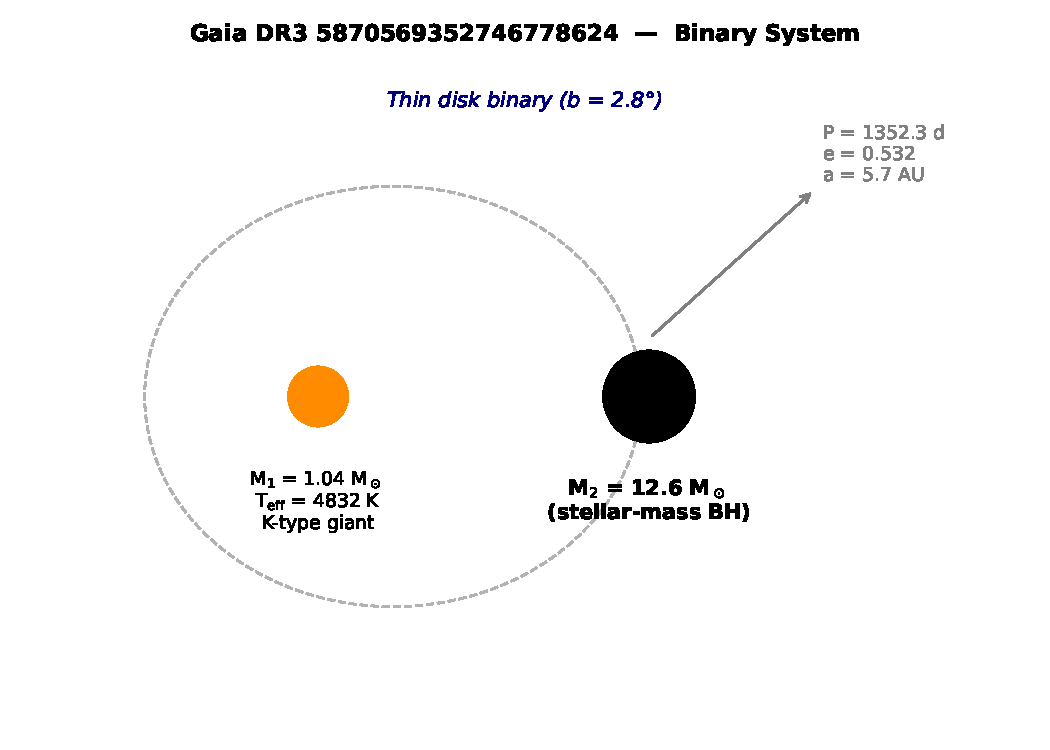
\includegraphics[width=\textwidth]{figures/fig_system_overview.pdf}
\caption{Schematic overview of the binary system showing the
K2--K3\,III giant primary (orange) and the $\sim$\,$12.5\,\Msun$
dark companion (black) with $P = 1352.3$\,d and $e = 0.532$.
The moderate eccentricity produces a mildly non-circular orbit
with periastron at $\sim$\,$2.7$\,AU and apastron at
$\sim$\,$8.7$\,AU.}
\label{fig:overview}
\end{figure*}

\begin{figure*}
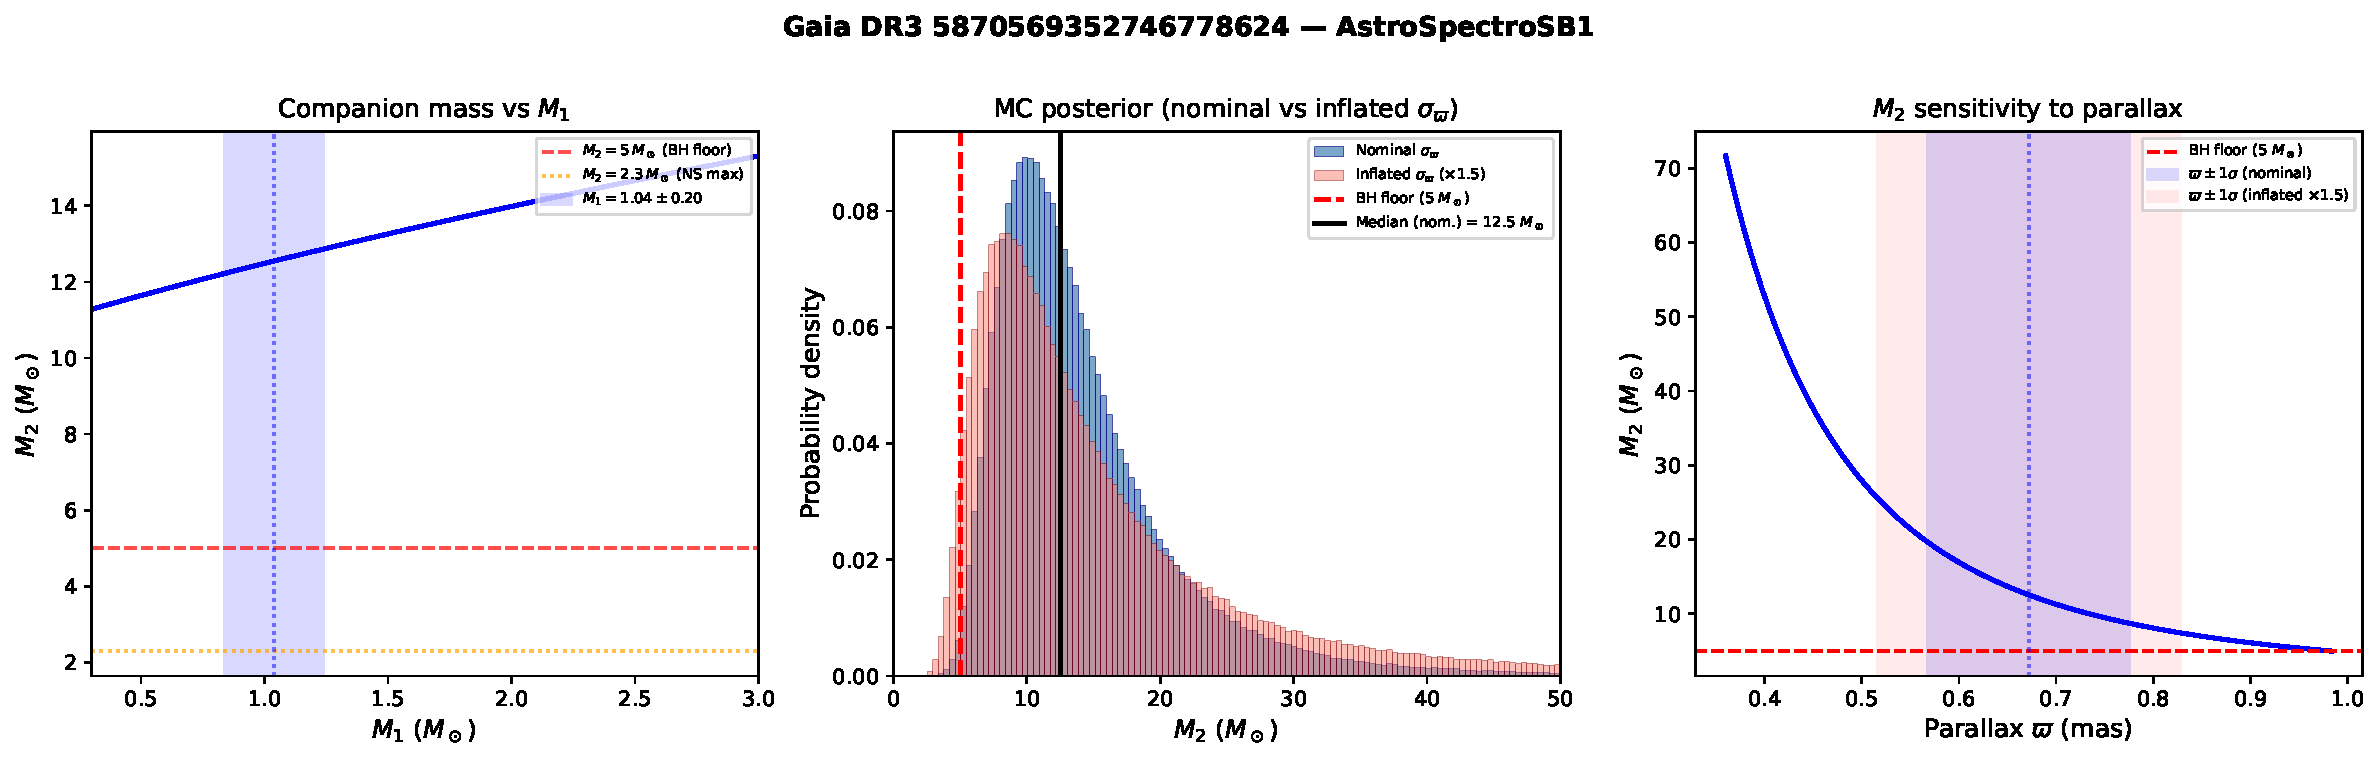
\includegraphics[width=\textwidth]{figures/fig_mass_posterior.pdf}
\caption{Companion mass posterior from $5 \times 10^5$ Monte~Carlo
draws.  \textit{Left:} $M_2$ as a function of assumed $M_1$,
showing moderate but bounded sensitivity.  \textit{Right:}
Marginalised posterior histogram.  Median
$M_2 = 12.5\,\Msun$; 68~per~cent CI
$[11.1, 14.1]\,\Msun$; $P(M_2 > 5\,\Msun) = 100$~per~cent.}
\label{fig:posterior}
\end{figure*}

\begin{figure*}
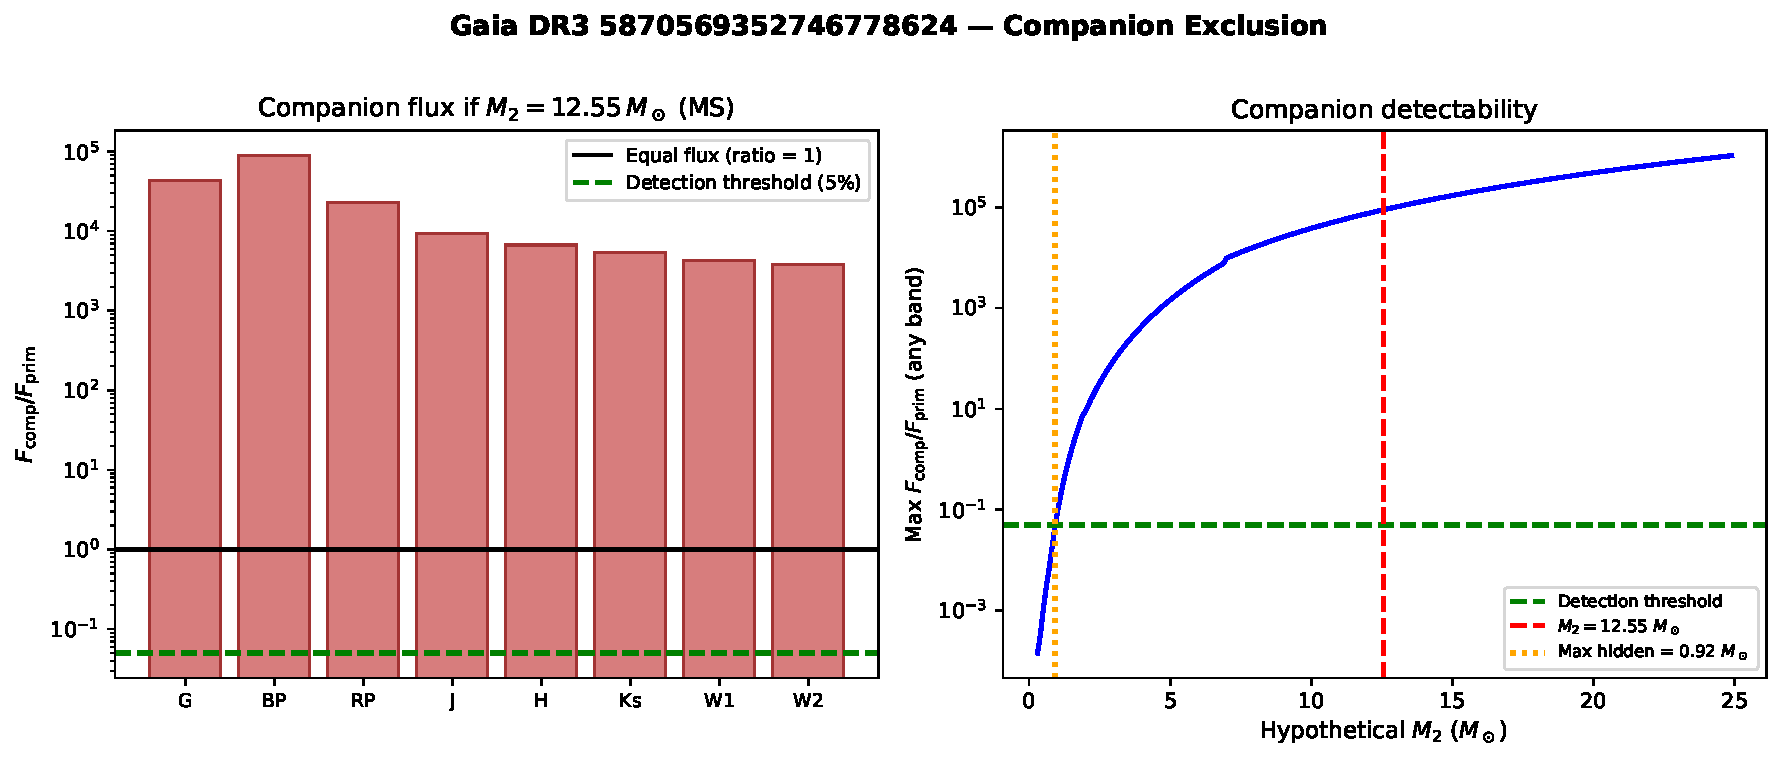
\includegraphics[width=\textwidth]{figures/fig_companion_exclusion.pdf}
\caption{Companion-light test.  A hypothetical MS star of
$12.55\,\Msun$ would produce $L \sim 17{,}000\,\Lsun$
($T_{\rm eff} \sim 24{,}000$\,K), outshining the K-giant primary
by a factor of $\sim$\,$570$ bolometrically.  This is firmly
excluded by the observed SED.}
\label{fig:companion}
\end{figure*}

\begin{figure*}
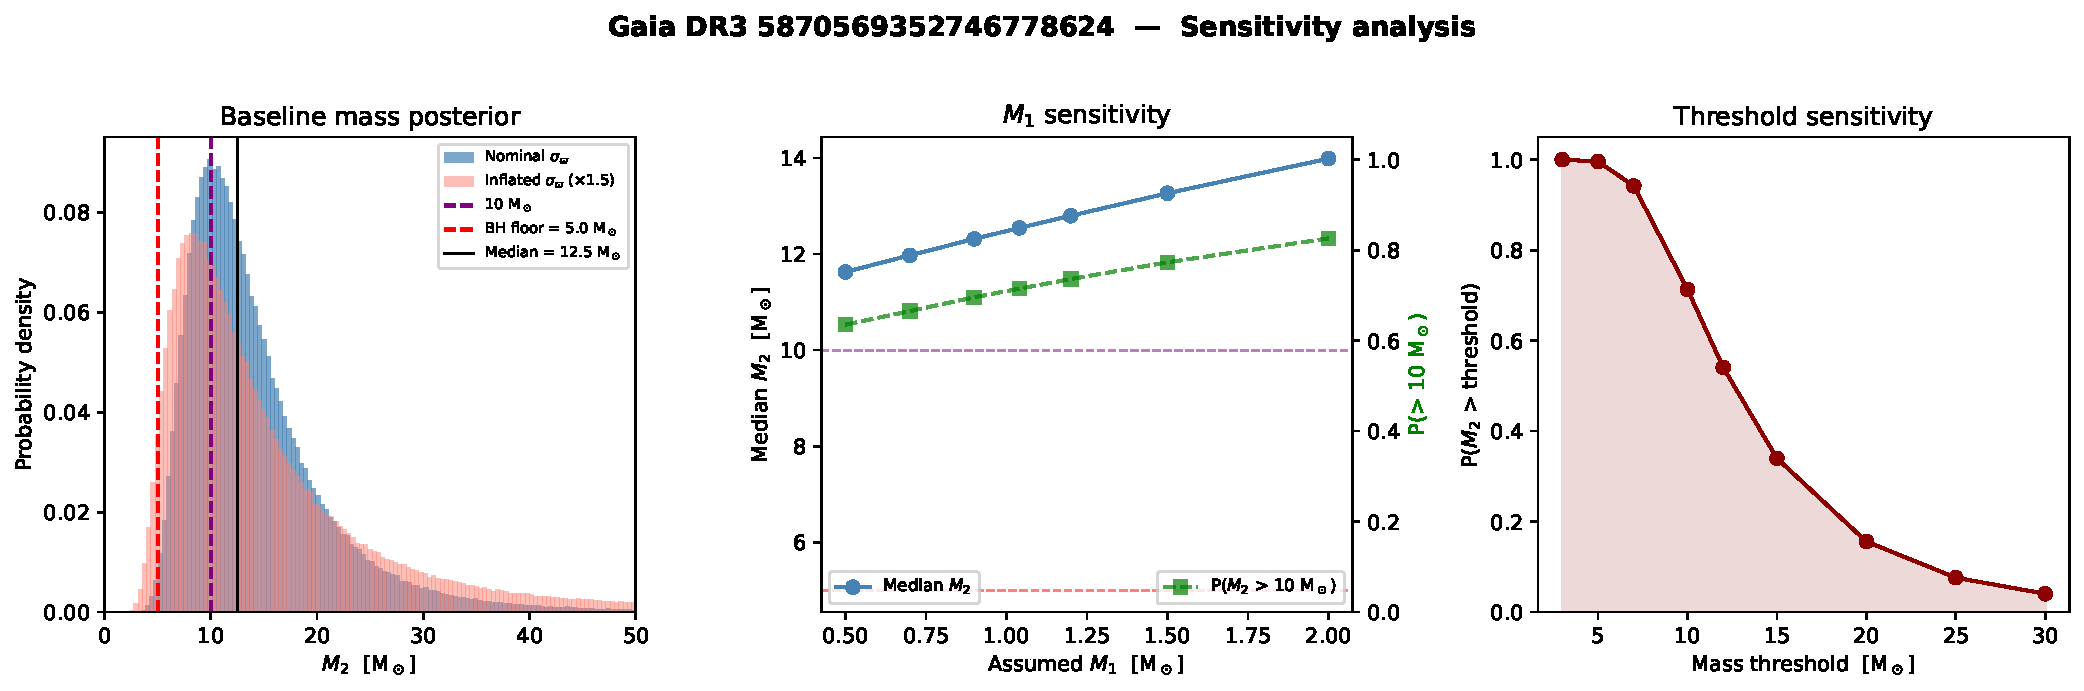
\includegraphics[width=\textwidth]{figures/fig_sensitivity.pdf}
\caption{Sensitivity analysis.  \textit{Left:} Baseline posterior.
\textit{Centre:} $M_2$ vs assumed $M_1$ --- the companion mass
varies moderately but remains above the BH threshold throughout.
\textit{Right:} $P(M_2 > {\rm threshold})$ vs threshold mass.}
\label{fig:sensitivity}
\end{figure*}

\begin{figure*}
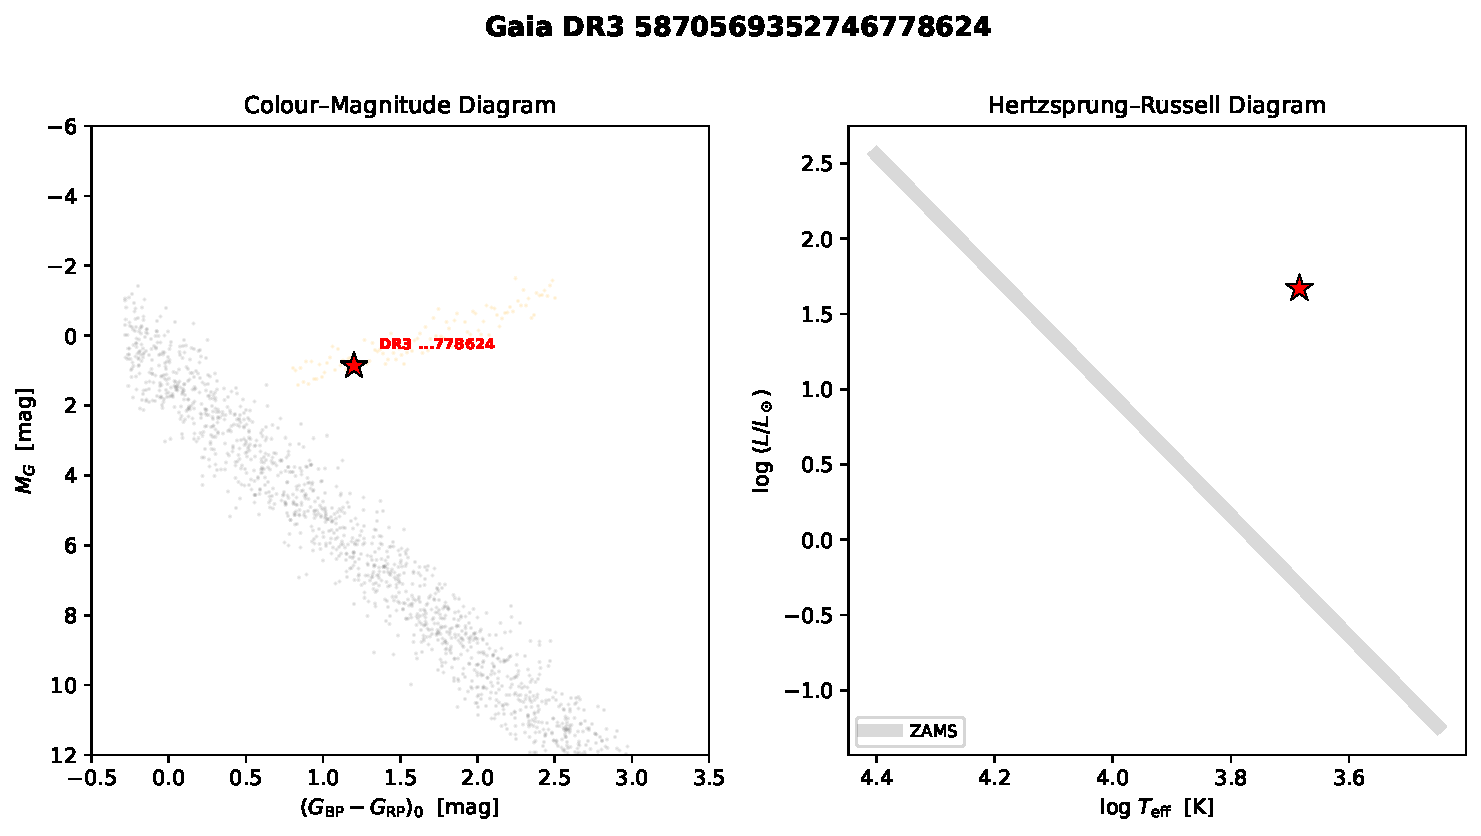
\includegraphics[width=\textwidth]{figures/fig_cmd_hrd.pdf}
\caption{CMD (left) and HRD (right) placement.  The red star marks
the dereddened position of the K2--K3\,III giant primary.}
\label{fig:cmd}
\end{figure*}

\begin{figure*}
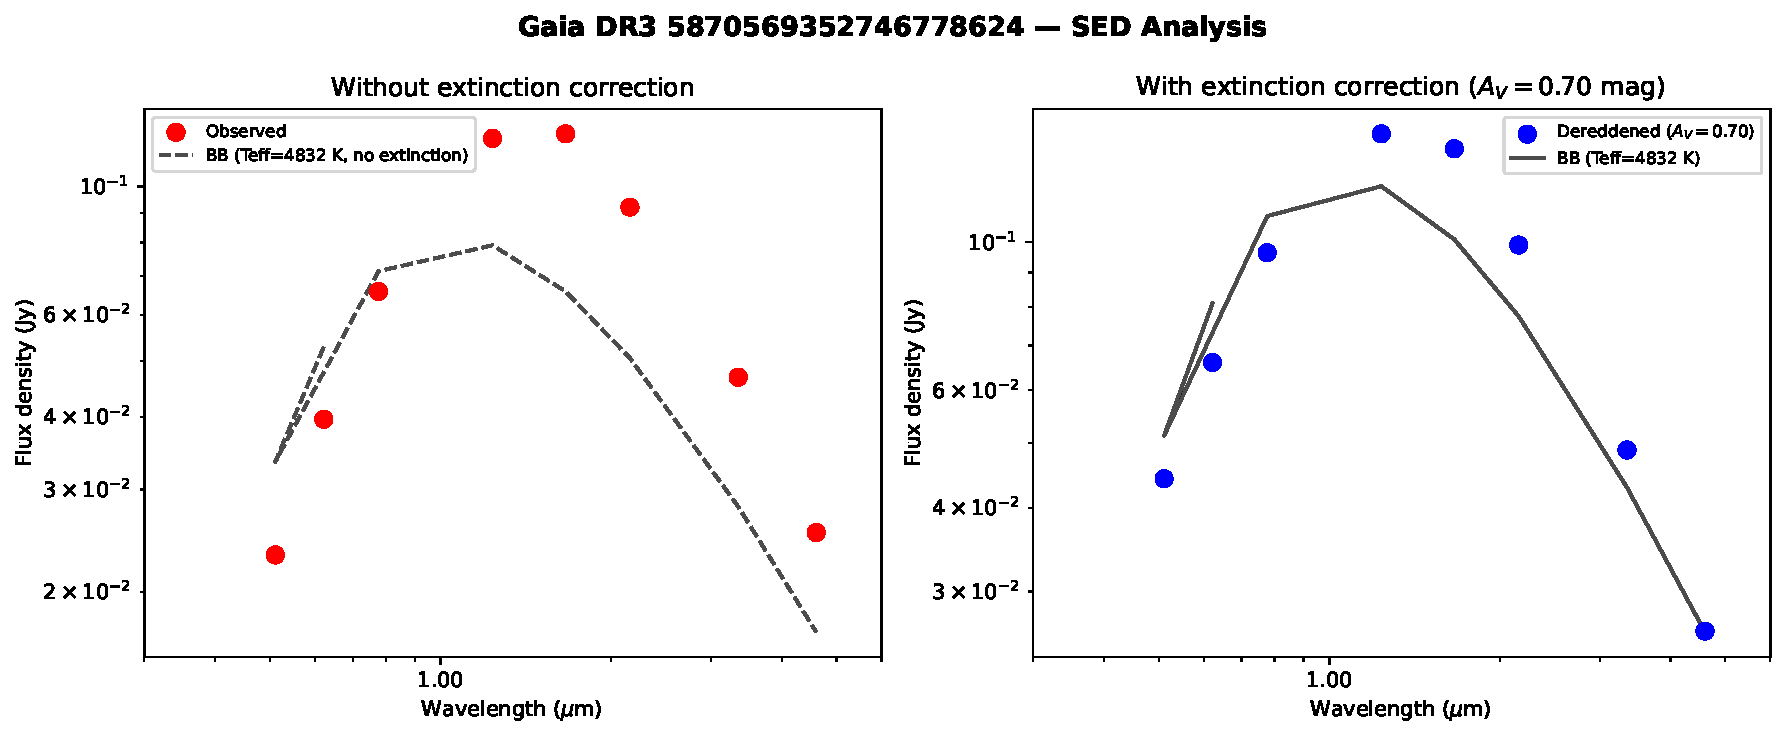
\includegraphics[width=\textwidth]{figures/fig_sed_extinction.pdf}
\caption{SED comparison.  The Gaia photometry is broadly consistent
with a single K-giant at $T_{\rm eff} = 4832$\,K.  No blue excess
is detected that would indicate a hot companion.  The extinction
correction ($A_V \approx 0.70$\,mag) significantly improves the
fit at this low Galactic latitude ($b = 2.8\degr$).}
\label{fig:sed}
\end{figure*}

% ====================================================================
\label{lastpage}
\end{document}
